\documentclass{extreport}

\usepackage[14pt]{extsizes}
\usepackage[T2A]{fontenc}
\usepackage[utf8]{inputenc}
\usepackage[english,ukrainian]{babel}

\usepackage[a4paper, top=10mm, bottom=15mm, left=20mm, right=15mm]{geometry}
\usepackage{amsmath,amsfonts,amssymb,amsthm,mathtools}
\usepackage{listings}
\usepackage{graphicx}
\usepackage{enumitem}
\usepackage{verbatim}
\usepackage{listings}
\usepackage{xcolor}
\usepackage{textgreek}
\usepackage{diagbox}
\usepackage{pgfplots}
\pgfplotsset{compat = 1.16}


\lstdefinestyle{output_txt}{
    basicstyle=\ttfamily\footnotesize,
    breakatwhitespace=false,         
    breaklines=true,                 
    captionpos=b,                    
    keepspaces=true,                                    
    numbersep=5pt,                  
    showspaces=false,                
    showstringspaces=false,
    showtabs=false,                  
    tabsize=2
}
\definecolor{codegreen}{rgb}{0,0.6,0}
\definecolor{codegray}{rgb}{0.5,0.5,0.5}
\definecolor{codepurple}{rgb}{0.58,0,0.82}
\lstdefinestyle{python_code}{ 
    commentstyle=\color{codegreen},
    keywordstyle=\color{magenta},
    numberstyle=\tiny\color{codegray},
    stringstyle=\color{codepurple},
    basicstyle=\ttfamily\footnotesize,
    breakatwhitespace=false,         
    breaklines=true,                 
    captionpos=b,                    
    keepspaces=true,                            
    numbersep=5pt,                  
    showspaces=false,                
    showstringspaces=false,
    showtabs=false,                  
    tabsize=4
}

\setlist[enumerate]{nosep}
\graphicspath{{pics/}}
\DeclareGraphicsExtensions{.png}

\begin{document}
\begin{titlepage}
    \thispagestyle{empty}
    \begin{center}
        
\includegraphics[width = \textwidth]{kpi}
        Міністерство освіти і науки України\\
        Національний технічний університет України\\
        <<Київський політехнічний інститут ім. І. Сікорського>>\\
        Інститут прикладного системного аналізу
    \end{center}
    \vspace{40mm}
    \begin{center}
        \textbf{Лабораторна робота} \\
        з курсу <<Методи оптимізації>> \\
        з теми <<Чисельні методи безумовної оптимізації другого порядку. 
        Метод Ньютона та його варіації>>
    \end{center}
    \vspace{20mm}
    \begin{flushleft}
        Виконали студенти 3 курсу групи КА-81 \\
        Галганов Олексій \\
        Єрко Андрій \\
        Фордуй Нікіта
    \end{flushleft}
    \begin{flushright}
        Перевірили \\
        Спекторський Ігор Якович \\
        Яковлева Алла Петрівна
    \end{flushright}
    \vspace{30mm}
    \begin{center}
        \textbf{Київ 2021}
    \end{center}
\end{titlepage}

\begin{center}
    \textbf{Варіант 1}
\end{center}
\textbf{Завдання.} Скласти програму для мінімізації цільової функції
одним з методів другого порядку (типу Ньютона). Конкретний тип методу обрати
самостійно, ураховуючи особливості цільової функції.

\emph{Цільова функція:}
$f(x,y) = x^2 + 18y^2 + 0.01xy + x - y$

\noindent\textbf{Результати роботи.}
Цільова функція є квадратичною, а тому використовувати узагальнені методи немає сенсу,
оскільки класичний метод Ньютона $x^{k+1} = x^k - [f''(x^k)]^{-1} f'(x^k)$
для строго опуклих квадратичних функцій знаходить розв'язок за одну ітерацію.
Доведемо це твердження. \\
Розглядаємо строго опуклі $f$ виду
$$f(x_1, ..., x_n) = \frac{1}{2}\left( A x, x\right) + \left(b, x\right) + c, \; A > 0$$
Тоді $$f'(x_1, ..., x_n) = Ax + b$$
$$ f''(x,y) = A$$
Нехай $x^0$ --- довільне початкове наближення, $x^*$ --- шуканий розв'язок, єдиний з умови строгої опуклості.
Запишемо перший крок метода Ньютона:
\begin{gather*}
    x^1 = x^0 - [f''(x^0)]^{-1} f'(x^0) \\
    x^1 = x^0 - A^{-1} \left( Ax_0 + b\right) \\
    x^1 = A^{-1}b
\end{gather*}
Отже, $x^1$ --- розв'язок рівняння $Ax+b=0$, що задає необхідну умову точки
мінімуму $f$. Відомо, що у випадку мінімізації опуклої функції на опуклій множині
(зокрема, на всьому просторі) необхідна умова мінімуму є достатньою.
Звідки отримуємо рівність $ x^1 =  x^*$, тобто точку мінімуму отримано після виконання одного кроку.$\qed$ 

Оскільки обраний критерій зупинки --- $\left| f(x_{k+1}) - f(x_k)\right| < \varepsilon = 10^{-5}$
вимагає принаймні дві ітерації для порівняння, було отримано збіжність до точки мінімуму за 2 ітерації.
\begin{center}
    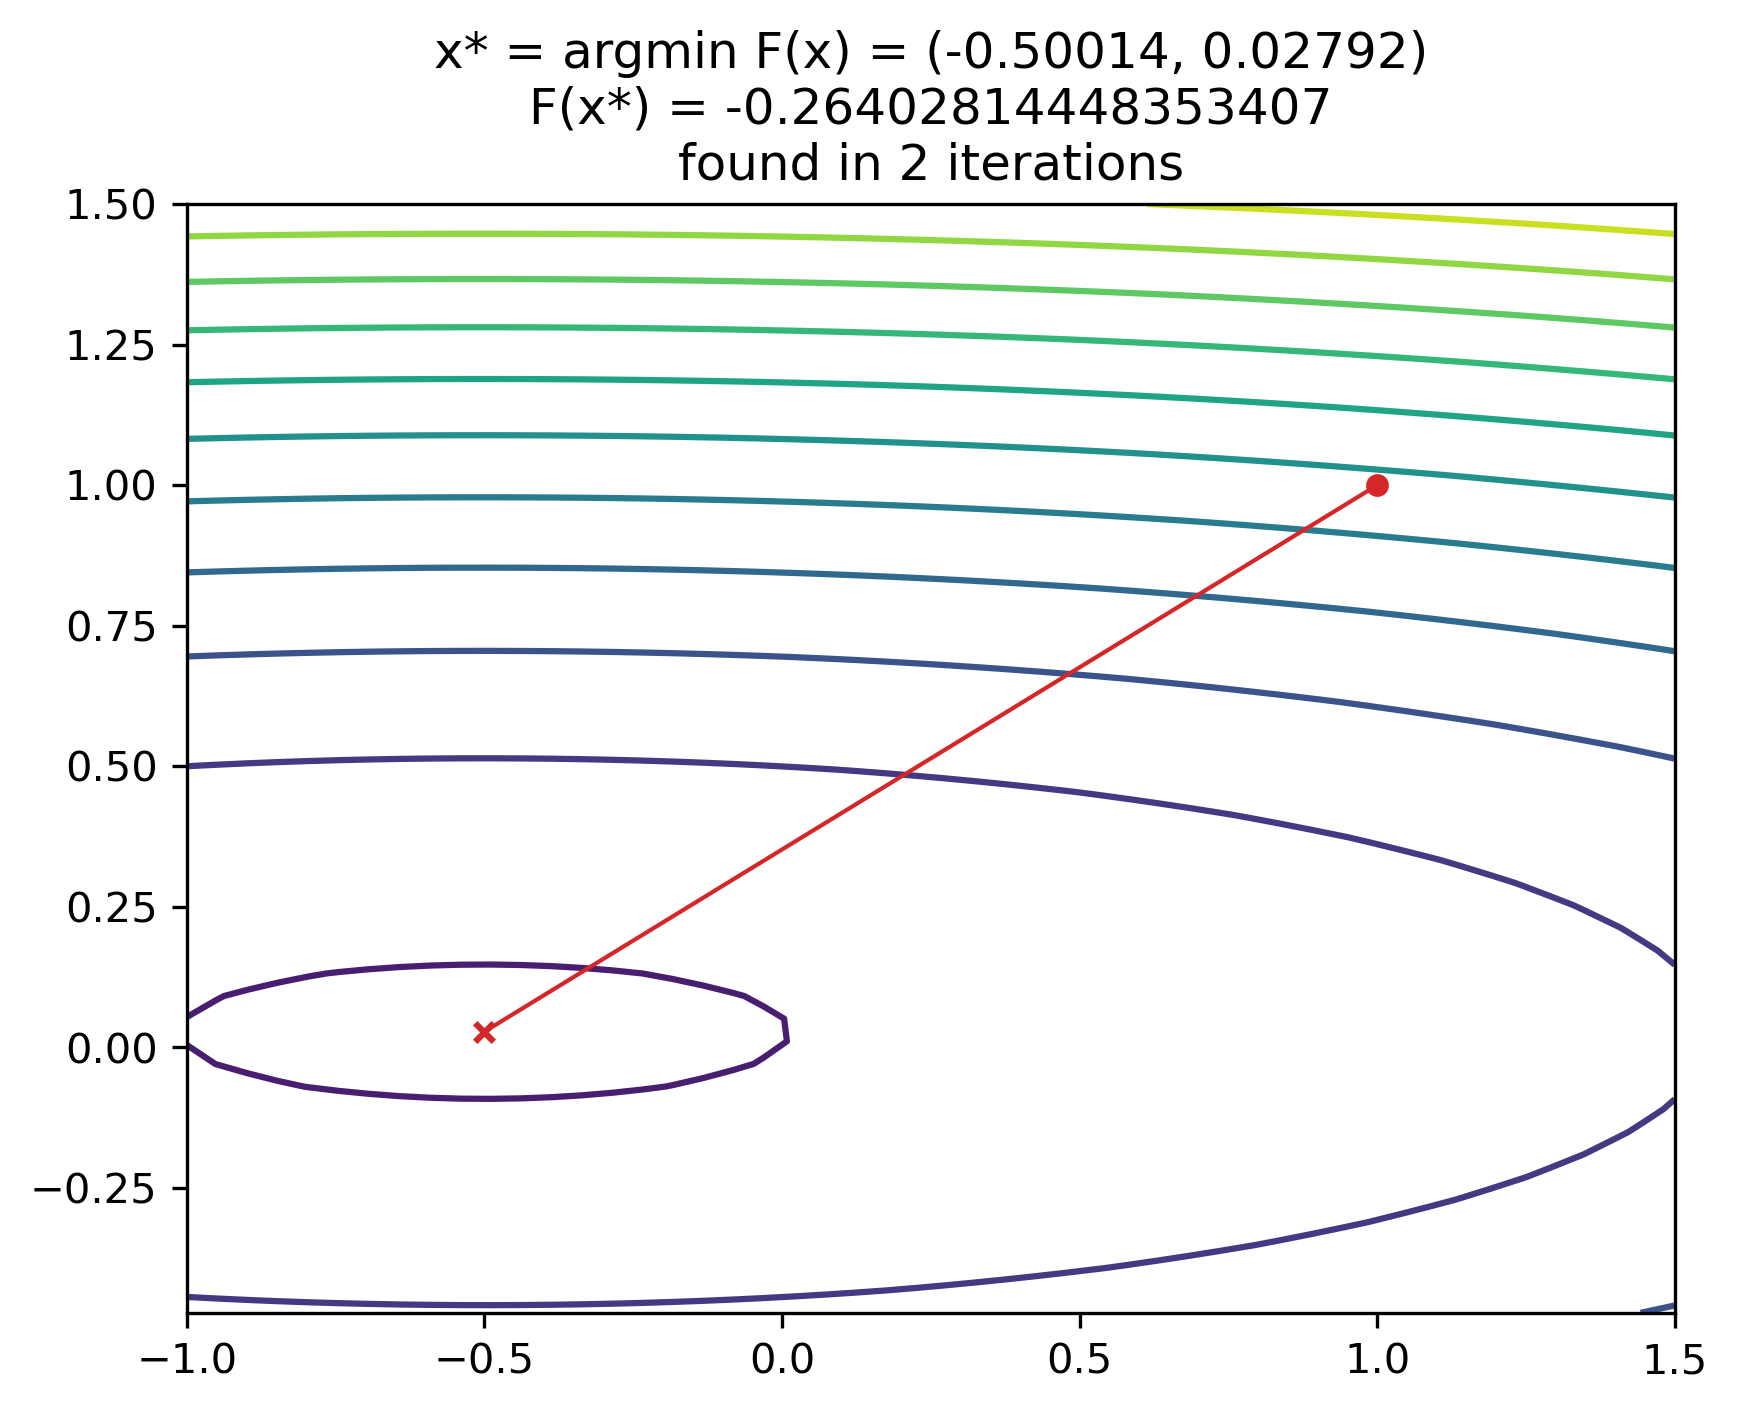
\includegraphics[scale = 0.8]{contour_final.png}
\end{center}

Перевіримо роботу реалізованої програми на функції $f(x, y) = (y - x^2)^2 + (1 - x)^2$,
що має мінімум у точці $(1, 1)$.
\begin{center}
    \begin{tabular}{|c|c|c|}
        \hline
        {} & \multicolumn{2}{c|}{кількість ітерацій}\\
        \hline
        $x_0$ & {класичний} & {узагальнений (дроблення кроку)}\\
        \hline
        $(1, 1)$ & 2 & 2 \\
        \hline
        $(10, 10)$ & 6 & 14 \\
        \hline
        $(100, 100)$ & 10 & 49 \\
        \hline
        $(1000, 1000)$ & 13 & 88 \\
        \hline
    \end{tabular}
\end{center}

\begin{center}

    \begin{tabular}{c c}
        {класичний} & {узагальнений (дроблення кроку)}\\
        \includegraphics[scale = 0.55]{result_(1.0, 1.0)_classic.png} &
        \includegraphics[scale = 0.55]{result_(1.0, 1.0)_frac.png} \\
        \includegraphics[scale = 0.55]{result_(10.0, 10.0)_classic.png} &
        \includegraphics[scale = 0.55]{result_(10.0, 10.0)_frac.png} \\
        \includegraphics[scale = 0.55]{result_(100.0, 100.0)_classic.png} &
        \includegraphics[scale = 0.55]{result_(100.0, 100.0)_frac.png} \\
        \includegraphics[scale = 0.55]{result_(1000.0, 1000.0)_classic.png} &
        \includegraphics[scale = 0.55]{result_(1000.0, 1000.0)_frac.png}
    \end{tabular}
\end{center}

\noindent\textbf{Лістинг.}
Текст програми було розділено на \texttt{Optimizer.py} з реалізацією
власне методу Ньютона та \texttt{lab2.py}, де він викликається та зберігаються результати.

\noindent\texttt{Optimizer.py}
\lstinputlisting[language = Python, style = python_code]{../code/Optimizer.py}

\noindent\texttt{lab1.py}
\lstinputlisting[language = Python, style = python_code]{../code/lab2.py}

\noindent\textbf{Висновки.} При виконанні даної роботи ми дослідили
застосування методу Ньютона до мінімізації заданої функції.
Оскільки мінімум строго опуклої квадратичної функції може бути знайдений класичним методом Ньютона
за одну ітерацію, було реалізовано саме його, а також --- доведено відповідний факт.
\end{document}